\section{Data and Monte Carlo Samples}
\label{sec:Files}

The CC inclusive studies reported here have included T2K Run 1-4 periods.  
In these studies we used 
production 5 ``Spin F''\footnote{ND280 software version v10r11p21} for Data and
production 5 ``Spin E''\footnote{ND280 software version v10r11p17} for the MC
samples. \\

We note that in the middle of both T2K Run 2 and T2K Run 4 
the \p0d water bags were drained.  
The results  presented in this report includes both 
%only the 
data periods when the \p0d water bags were empty and filled with water.  
%(both in Run 1 and Run 2.)

\subsection{Data Sample} 

\begin{table}[h]
\centering
\begin{tabular}{cccc}\toprule
\multirow{2}{*}{Data Set} & \multirow{2}{*}{Run Period} & \multicolumn{2}{c}{Protons On Target}\\
 & & Total (Available) & DQ (Used) \\
\hline
Run 1 & Jan 2010 - Jun 2010 & $3.033\times 10^{19}$ & $2.946 \times 10^{19}$\\ 
Run 2 & Nov 2010 - Feb 2011 & $6.974\times 10^{19}$ & $4.286 \times 10^{19}$\\ 
Run 4 & Oct 2012 - Feb 2013 & $16.45\times 10^{19}$ & $16.24 \times 10^{19}$\\ 
\hline
Total &  & $26.46 \times 10^{19}$ & $23.47 \times 10^{19}$ \\ 
\bottomrule
\end{tabular} 
\caption{The POT values available and used in the data analysis for 
the Water-in run periods}
\label{tab:DataSamplesRun1Run2Run4} %FIXME
\end{table}

The total number of Protons On Target (POT) recorded in the four T2K periods 
was $\sim62.18\times 10^{19}$ POT. 
The \p0d Water-in periods included $\sim 27.95\times 10^{19}$ POT and
the \p0d Water-out periods included $\sim 34.23\times 10^{19}$ POT. \\

The studies presented here have incorporated 
both the ``ND280'' Data Quality flag and the beam ``GoodSpill" flag checks. 
After these checks, the Water-in analyses included 11,237 SubRuns 
that sum up to around $23.47\times 10^{19}$ POT and 
the Water-in analyses included 12,255 SubRuns 
that sum up to around $33.54\times 10^{19}$ POT.
The breakdown for the different run periods is shown 
in Tables \ref{tab:DataSamplesRun1Run2Run4} 
and \ref{tab:DataSamplesRun2airRun3airRun4air} for the 
Water-in and Water-out respectively. \\

\begin{table}[h]
\centering
\begin{tabular}{cccc}\toprule
\multirow{2}{*}{Data Set} & \multirow{2}{*}{Run Period} & \multicolumn{2}{c}{Protons On Target}\\
 & & Total (Available) & DQ (Used) \\
\hline
Run 2 & Feb 2011 - Mar 2011 & $3.593\times 10^{19}$ & $3.552 \times 10^{19}$\\ 
Run 3 & Apr 2012 - Jun 2012 & $13.58\times 10^{19}$ & $13.48 \times 10^{19}$\\ 
Run 4 & Feb 2013 - Aug 2013 & $16.37\times 10^{19}$ & $15.86 \times 10^{19}$\\ 
\hline
Total &  & $33.54 \times 10^{19}$ & $32.89 \times 10^{19}$ \\ 
\bottomrule
\end{tabular} 
\caption{The POT values available and used in the data analysis for 
the Water-in run periods}
\label{tab:DataSamplesRun2airRun3airRun4air} %FIXME
\end{table}

\subsection{Monte Carlo Sample} 

Dedicated Monte Carlo samples were 
produced for the different T2K run periods. 
These samples incorporated the different detector configurations 
and the different beam flux profile when weighted.
The main change Run 1 and the other run periods 
in the detector configuration was the addition
of the Barrel ECal.
In addition, Run 3 and Run 4 MC samples are assume higher beam power 
which results in more simulated events per POT.
The exact amount of MC files used for each run period and their 
corresponding POT is shown in Table \ref{tab:MCSamplesRun1Run2Run4} and 
Table \ref{tab:MCSamplesRun2airRun3airRun4air} 
for the Water-in and Water-out respectively. \\

\begin{table}[h]
\centering
\begin{tabular}{ccc} \toprule
MC Configuration & Number of files & Protons On Target \\
\hline
Run 1 & 1,102 & $55.10 \times 10^{19}$ \\ 
Run 2 & 1,483 & $75.15 \times 10^{19}$ \\ 
Run 4 & 9,863 & $496.2 \times 10^{19}$ \\ 
\hline
Total &  &$625.4 \times 10^{19}$ \\ 
\bottomrule
\end{tabular} 
\caption{The available Water-in MC samples and their corresponding 
POT used for the Water-in analysis}
\label{tab:MCSamplesRun1Run2Run4} %FIXME
\end{table}

In the analysis we compared the different data run periods   
separately to the different MC samples generated by NEUT \cite{neut}. 
These generated samples consist of neutrino interactions created 
in the whole ND280 detector volume which includes the magnet region.
NNN 
In addition we have used the Production 4 `Sand interaction' MC sample 
which contains 700 files that are equivalent to $\sim7\times 10^{19}$ POT 
and should include interactions that occur, 
in the surrounding pit and soil area.

\begin{table}[h]
\centering
\begin{tabular}{ccc} \toprule
MC Configuration & Number of files & Protons On Target \\
\hline
Run 2 & 1,991 & $99.55 \times 10^{19}$ \\ 
Run 3 & 3,221 & $161.1 \times 10^{19}$ \\ 
\hline
Total &  &$260.6 \times 10^{19}$ \\ 
\bottomrule
\end{tabular} 
\caption{The available Water-in MC samples and their corresponding 
POT used for the Water-in analysis}
\label{tab:MCSamplesRun1Run2Run4} %FIXME
\end{table}

 
\subsection{Weighting by beam flux} 

The Production 5 MC files were generated by GENIE and NEUT, 
which depend on beam MC using the 11a (version 2) of Jnubeam. 
To account for external hadron production data 
from the NA61 experiment and other experiments, 
inputs (e.g.~actual proton beam information) 
are incorporated by the Beam Group
to reweight the neutrino beam flux as a function of neutrino energy. 
The Beam Group releases
this information as a set of histograms that include 
the ratio of tuned to nominal flux histograms. 
We use the true neutrino energy of each MC event and the `tuned to nominal' 
ratio histogram to reweight that event.
The current analysis utilizes the 11b version 3.2 tuned flux ratios.
These `tuned to nominal' ratios as a
function of true neutrino ($E_{\nu}$) energy are shown 
in Fig. \ref{fig:TunedfluxRatio}.

\begin{figure}
\centering
\subfloat[Run 1 Ratio]{
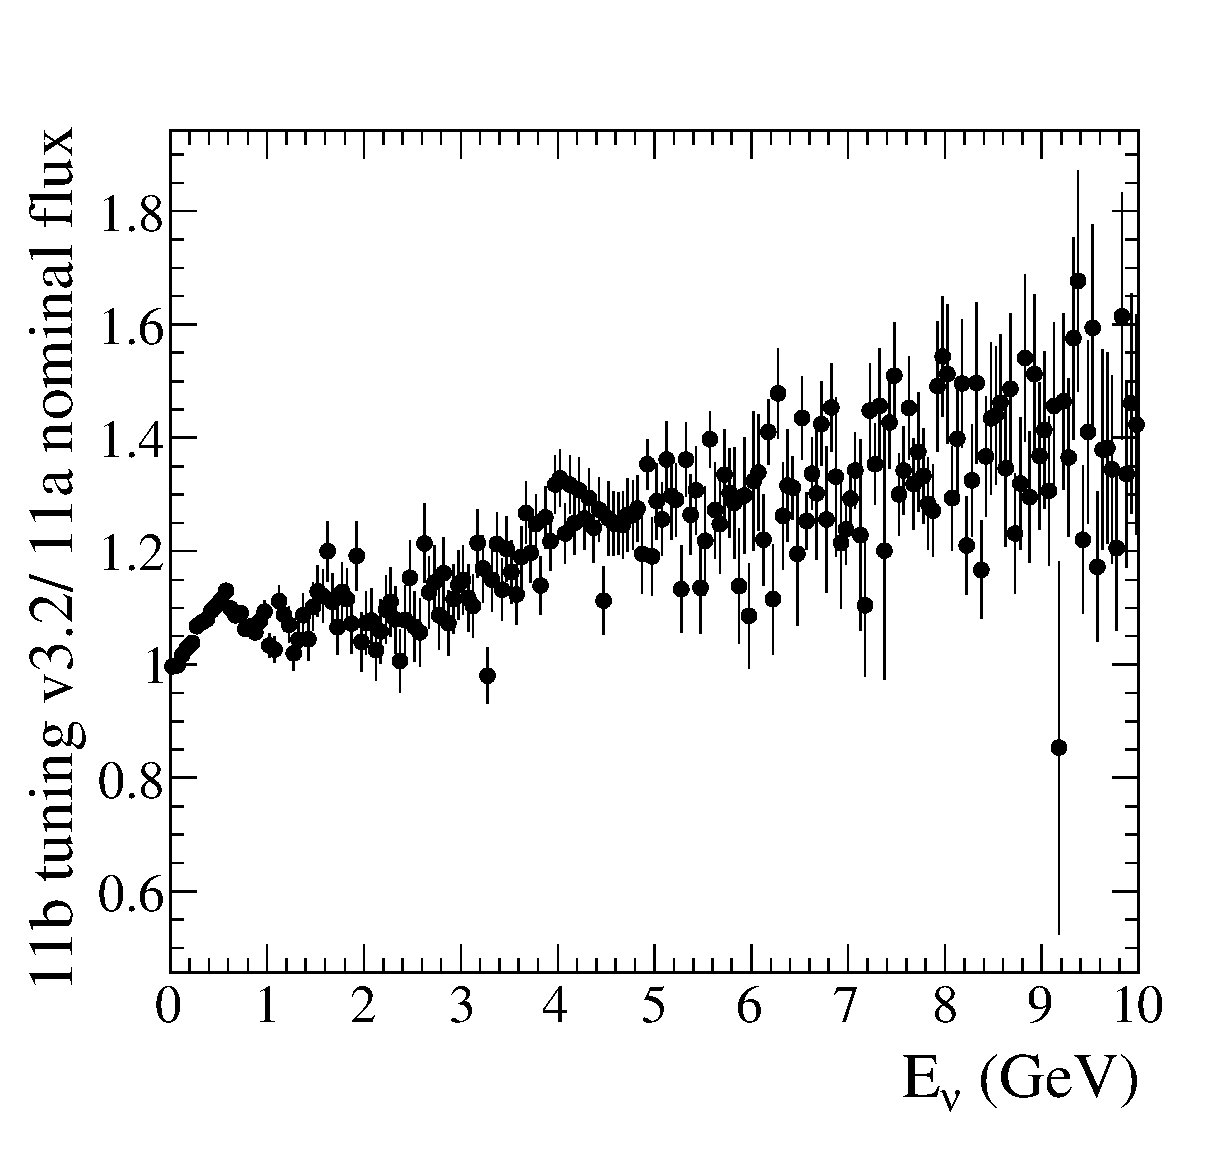
\includegraphics[width=0.48\textwidth]{Figures/run1-fluxreweight.eps}
}
\subfloat[Run 2 Ratio]{
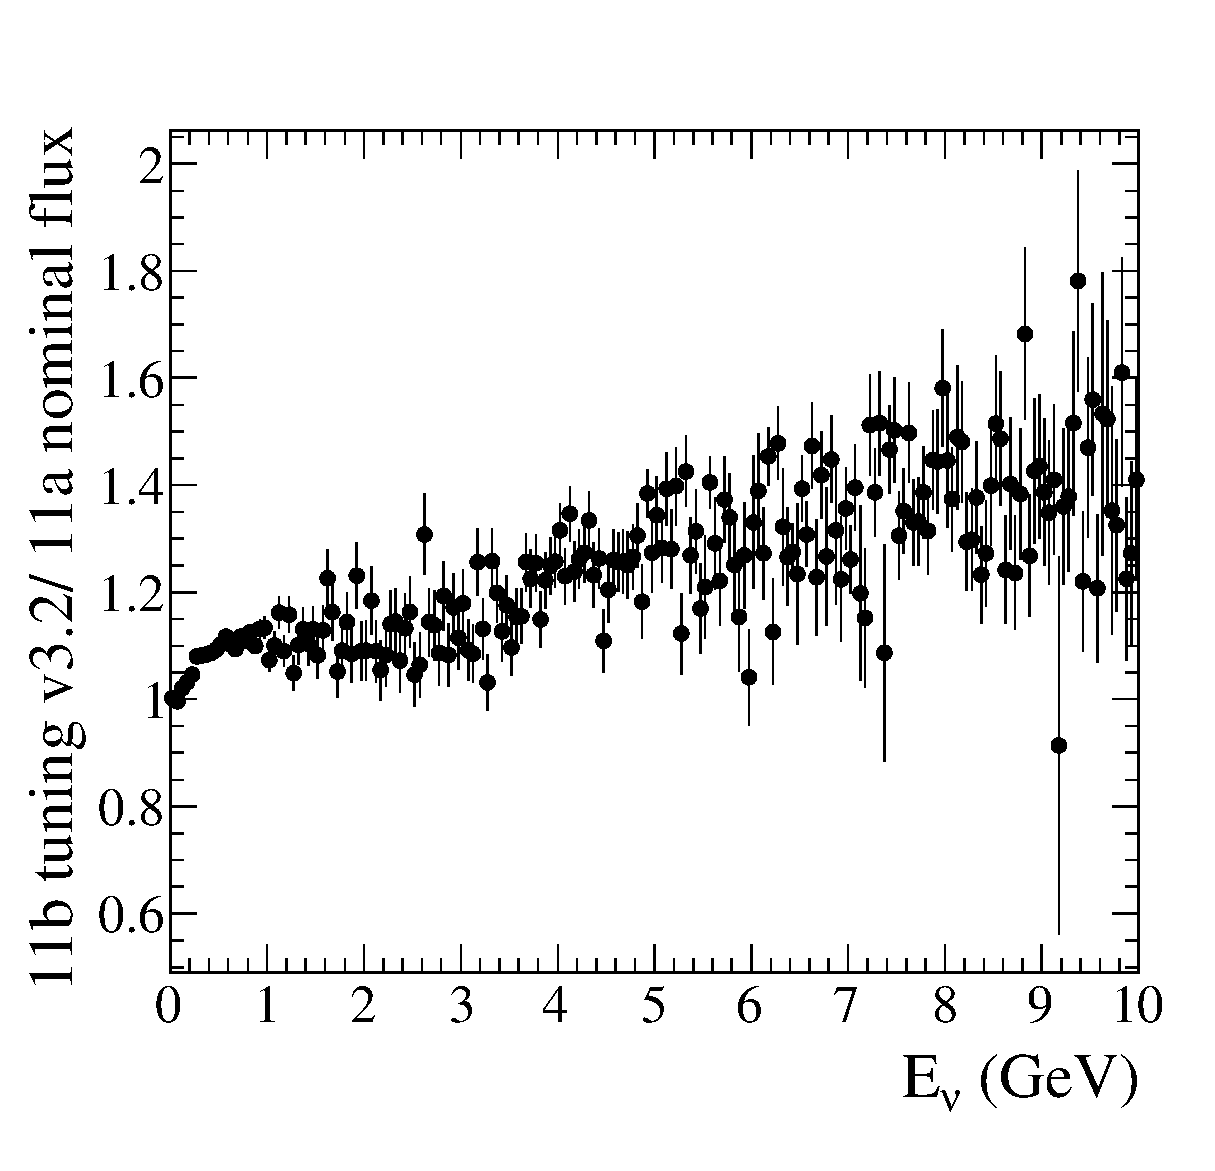
\includegraphics[width=0.48\textwidth]{Figures/run2-fluxreweight.eps}
}
\caption{The 11b version 3.2 tuned to nominal flux ratios}
\label{fig:TunedfluxRatio}
\end{figure}

